\documentclass[8pt]{article}
\usepackage[utf8]{inputenc}    % For UTF-8 character encoding
\usepackage[T1]{fontenc}       % For proper font encoding
\usepackage{lmodern}           % Improved font rendering
\usepackage{amsmath, amssymb}  % For math symbols and environments
\usepackage{graphicx}          % For including images
\usepackage{geometry}          % For adjusting page dimensions
\usepackage{hyperref}          % For clickable hyperlinks in the document
\usepackage{fancyhdr}          % For custom headers and footers
\usepackage{parskip}           % To add space between paragraphs
\usepackage{tikz}              % For drawing figures
\usepackage{booktabs}          % For improved table formatting
\usepackage{enumitem}          % For custom lists
\usepackage{caption}           % For customizing captions
\usepackage{listings}          % For code listings
\usepackage{multirow}          % For multirow tables

\lstset{
  frame=tb,
  language=C,
  aboveskip=3mm,
  belowskip=3mm,
  showstringspaces=false,
  columns=flexible,
  basicstyle={\small\ttfamily},
  numbers=none,
  numberstyle=\tiny\color{gray},
  keywordstyle=\color{blue},
  commentstyle=\color{brown},
  stringstyle=\color{orange},
  breaklines=true,
  breakatwhitespace=true,
  tabsize=3
}
\usepackage{amsmath}
\usepackage{tikz}
\usetikzlibrary{automata, positioning}

\begin{document}

\pagestyle{fancy}
\fancyhf{}
\fancyhead[L]{\leftmark} % Left header contains the section name
\fancyhead[R]{\thepage}  % Right header contains the page number

\title{Document Title}
\author{WANG Xiyu}
\date{\today}
\section*{DFA for the Language \( L = \{ w \in \{0, 1\}^* \mid \textrm{w ends with } 01 \} \)}

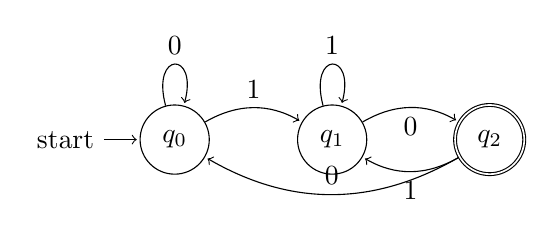
\begin{tikzpicture}[shorten >=1pt, node distance=2cm, on grid, auto]
   \node[state, initial] (q_0)   {$q_0$}; 
   \node[state] (q_1) [right=of q_0] {$q_1$}; 
   \node[state, accepting] (q_2) [right=of q_1] {$q_2$};

    \path[->] 
    (q_0) edge [loop above] node {0} ()
          edge [bend left, above] node {1} (q_1)
    (q_1) edge [bend left, below] node {0} (q_2)
          edge [loop above] node {1} ()
    (q_2) edge [bend left, below] node {1} (q_1)
          edge [bend left, above] node {0} (q_0);
\end{tikzpicture}

\section*{Example: Tut 1 Q4}
\subsection*{DFA for the Language \( L = \{ s \in \{a, b\}^* \mid \textrm{s does not contain substring 'ababba'}  \} \)}


\end{document}
